\section{Results}
\begin{figure}
	\centering
    \resizebox{\columnwidth}{!}{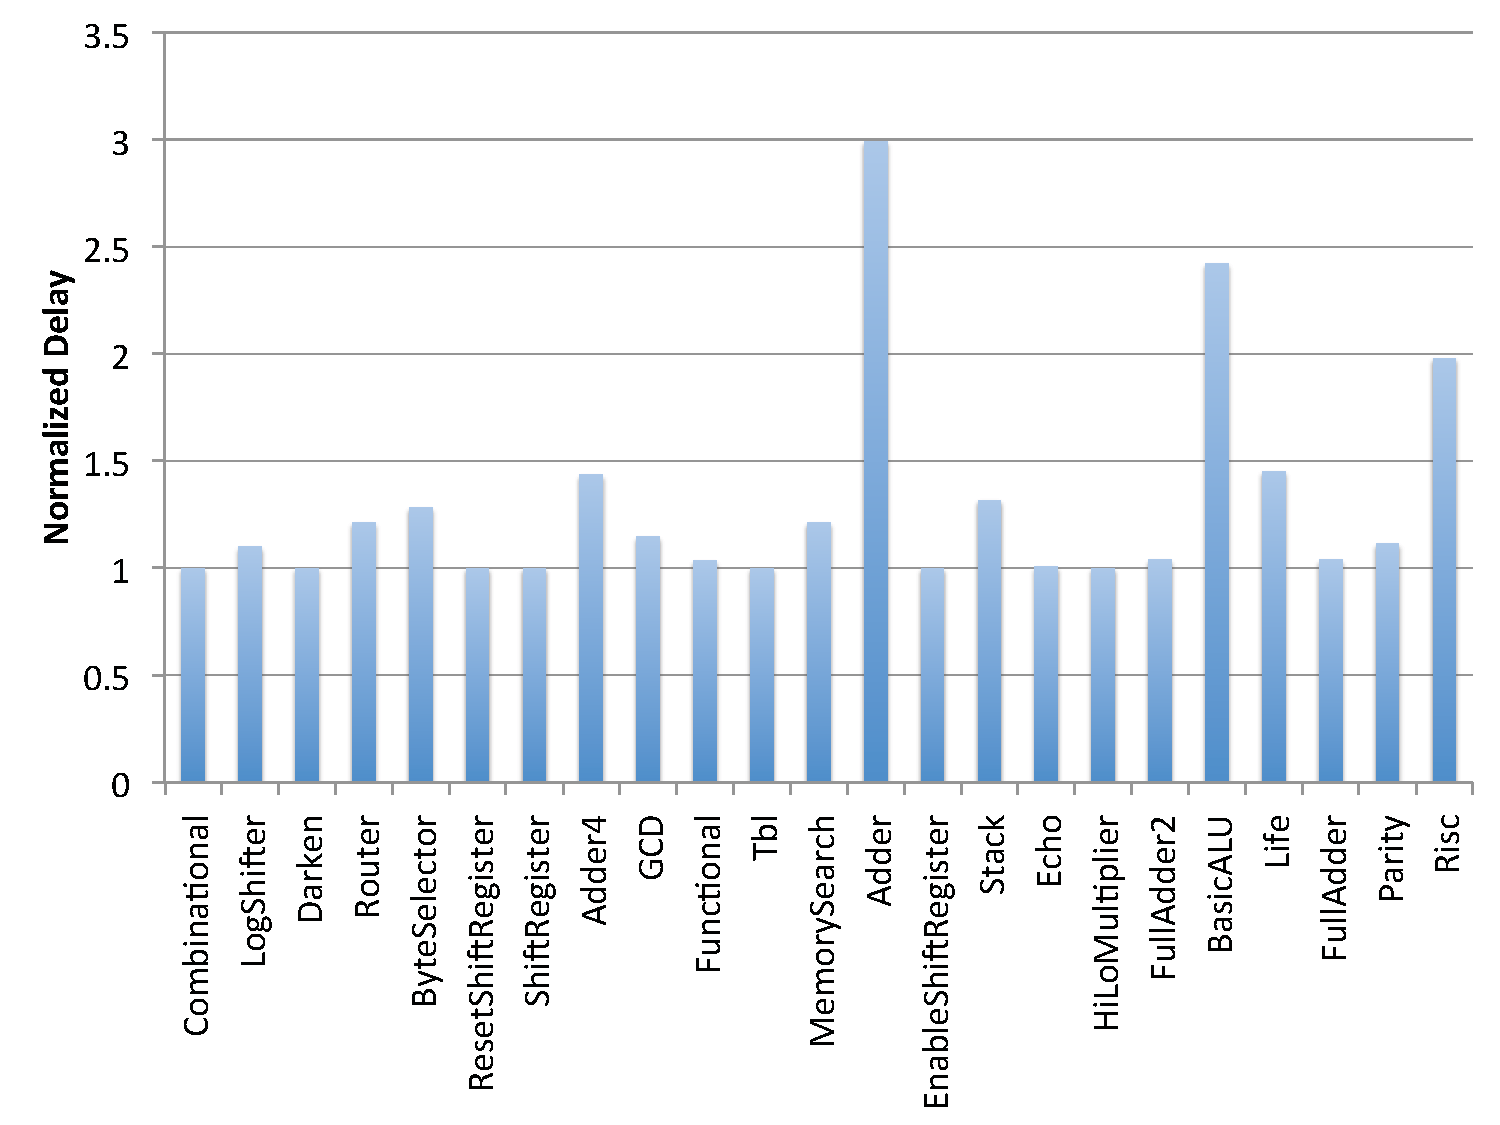
\includegraphics{figures/backannotation_result}}
    \caption{The critical path delays from the Chisel backannotator normalized to those from Design Compiler. We use example Chisel designs in the Chisel tutorial}
	\label{backresult}
\end{figure}
\subsection{Chisel Backannotation}
To verify the Chisel backannotator, we compare the critical path delays from the Chisel backannotator with those from Design Compiler. Figure \ref{backresult} shows thecritical path delays calculated by the Chisel backannotator normalized to those calculated by Design Compiler. Design Compiler executes with minimal optimizations, which only checks hold time constraints. With the ideal Chisel backannotator, the normalized critical path delays should be 1.

However, the inaccuracies of the Chisel backannotation mainly come from delay estimation for missing signals presented in Section \ref{challenges}. It is possible for a Chisel node to have a delay number greater than its actual delay. For example, suppose there are only two timing paths P1 and P2. P1 is a path from X through T1, T2, and T3 to Y, and P2 is a path from X through T1 and T4 to Y where T1, T2, T3, and T4 are missing signals. We also assume that the delay of P1 is 4 and the delay of P2 is 3.9. In this case, the critical path is P1 whose delay is 4. The delay estimation by the Chisel backannotator for T1, T2, T3, and Y is 1 when reading the timing report of P1, while that of T1, T4, and Y is 1.3 when reading the timing report of P2. The Chisel backannotator then selects 1.3 as the delay of T1 and Y and concludes the critical path is 4.6. This explains why many designs such as Adder, BasicALU, Risc, and Life have a normalized delay much greater than 1.

To be worse, the fact that a design has a normalized delay equal to 1 does not mean each Chisel node has the exact delay number. The critical path delay from the Chisel backend might be close to that from Synopsys tools although each node has different delays. This is highly likely to happen due to the naive delay estimation of the Chisel backend. Thus, we need more elaborated verification method for the Chisel backannotator.

\subsection{Automatic Pipeline Register Placement}
We first want to evaluate the automatic pipeline placement independently from the Chisel Backannotation. Thus, we first run a very simple finite state machine, a simple RISC processor, and the Sodor processor through the automatic pipeline tools using mock delay numbers.  The metric of interest is the ratio of the maximum combinational path delay after optimization to unpipelined combinational path delay/number of stages. This is a useful metric because the unpipelined combinational path delay/number of stages tells us the best possible maximum path delay the automatic pipelining tool can achieve given the specified number of stages. Insert Table here:

As seen in the Figure x, the automatic pipeline tool achieves close to optimal placement on a very simple finite state machine, relatively good placement on a simple RISC processor, and the worst placement on the Sodor processor. This trend is explained by the fact that the automatic pipelining tool is more constrained on where it can place the pipeline registers on the more complex designs. Several things constrain the placement of the pipeline registers:

{\bf (1)} 
As discussed previously, the tool is not allowed to move IO nodes across pipeline stage boundaries. In more complex designs, there are more IO nodes and they prevent not only themselves, but also their inputs and consumers from being freely placed by the automatic pipelining tool. In the case of input nodes, its consumer nodes must be placed at a stage {\tt >=} the stage of the input node. In the case of output nodes, its input nodes must be placed at a stage {\tt <=} the stage of the output node.

{\bf (2)}  
The automatic pipelining tool cannot put pipeline registers in the middle of large black box modules such as caches. Thus, if the delay across the black box module is the critical path delay, the tool cannot reduce the critical path delay any further. The simple finite state machine does not use any black box modules while the more complex designs do.

{\bf (3)} 
The automatic pipelining tool cannot put pipeline registers between the input and output muxes of the read and write ports of array memories. In some designs, these read and write ports of array memories is a significant portion of the unpipelined critical path delay and thus the tool is unable to reduce the critical path delay below the propagation delay through the read and write ports of the array memories. The simple finite state machine does not use any array memories while the more complex designs each have an array memory for the register file.
\subsection{Combined Tool Results}

